%----------------------------------------------------------------------------------------
%----------------------------------------------------------------------------------------
%----------------------------------------------------------------------------------------
%Method
%----------------------------------------------------------------------------------------
%----------------------------------------------------------------------------------------
%----------------------------------------------------------------------------------------

\section{METHOD}
\label{sec: method}
\subsection{Choosing an Algorithm}

Some of the most tested methods of data mining in astronomy are artificial neural networks (ANNs)~\citep[e.g.][and references therein]{Hossein14,Hossein16}.
ANNs are designed to work in the same way that the neurons work in a human brain.
These are networks of interconnected neurons (nodes), in which all of the connections are weighted.
These networks are used to study nonlinear and complex relations between input and output data.
One of the most well-known unsupervised neural networks in astronomy is a Kohonen self-organizing map (also called self-organizing map, or SOM).
SOMs visualize complex data~\citep{Kohonen82} and show simple geometrical relationships in non-linear high dimensional data~\citep{Kohonen98}.
The result of a SOM is a 1D or 2D network of neurons, which shows the positions of clusters and their relative distance.
Since the 1990s, many studies utilized SOMs for object classification and clustering (e.g. classifying quasars' spectra, star/galaxy classifications, gamma-ray burst clustering and light curve classification) and photometric redshift estimation~\citep[e.g.][]{Odewahn92, Hernandez94, Murtagh95, Maehoenen95,Scaringi09,Geach12,Fustes13,Meusinger16,Rahmani16b} %%% Why I cannot add submitted in front of the high-z paper %PB: MNRAS style guide says "Private communications or papers in preparation should be listed as such in the text, but omitted from the reference list, e.g. Smith (in preparation) shows that… " -- but I'm not clear on whether this applied to submitted papers or not

K-means algorithm, SOMs, and hierarchical clustering are the main unsupervised methods that are used in astronomical studies~\citep[e.g.][]{DAbrusco12, Aycha16}. %%add one or two more
For both K-means and SOM algorithms, the user must define the number of clusters, and the algorithms decide how to separate the data into the desired number of clusters.
In the hierarchical clustering method, the user must define dissimilarity between the groups; the algorithm combines (or divides) existing groups based on their dissimilarity and creates a hierarchical structure. 
Comparing the SOMs, K-means and hierarchical clustering methods shows that in some cases the hierarchical clustering method mis-classifies the data~\citep[][and references therein]{Mangiameli96}.
We chose the SOM method over K-means method due to the fact that SOMs not only cluster data, but also show similarities and dissimilarities between the clusters.
Therefore, we can cluster our sample data and study the underlying structure simultaneously.

 \subsection{Self Organizing Maps}
 \label{sec: som}
 The SOM is a clustering method which reduces the dimensionality of data, while preserving topological features~\citep{Kohonen98}. 
 The results of the SOM are shown with a map of neurons, which their numbers are set by the user.
 Each neuron has a fixed position in the map and may contain one or more samples from the input data,~\boldit{V} $\in \Re^n$. % Els said the simbols should be describe?! I think it is pretty obvious!
 A weight vector,~\boldit{W} $\in \Re^n$, with the same dimension as the input data, is associated with each node and will be varied during the training process.
 The process of creating an SOM happens over a series of $N$ iterations.
 In each iteration, the algorithm calculates the Euclidean distance for each node $j$ as $D_j^2= \sum_{i=0}^{i=n} (V_i - W_i)^2$, and finds a neuron with $D_{j_,{\mathrm min}}$. 
 This neuron is the winner node and is calling Best Matching Unit (BMU). 
 The weight vectors in the neighbourhood of the BMU will change according to the Kohonen learning rule (equation~\ref{equ: weight adj}). 
  \begin{equation}
            \label{equ: weight adj}
            W(t+1)=W(t)+L(t) \times R(t) \times(V(t)-W(t))
 \end{equation}
where $L(t) = L_0 e^{(-t/\tau)}$ is the learning factor, which prevents the divergence of the SOM, and $R(t)=\exp(-\frac{D_j^2}{2r^t_{BMU}})$ is the influence rate, which determines how the weight of each node will change.
Values for the number of neurons, $L(t)$ and $R(t)$ are arbitrary. 
~\cite{Geach12} and \cite{Rahmani16b} demonstrate the algorithm of the SOM in more detail.


     In order to create self-organizing maps, we used the \textsc{matlab} neural network toolbox~\citep[NNT,][]{matlabtolbox}.
     An SOM in \textsc{nnt} can be created by the \textsc{newsom} library which works in two phases, the ``ordering phase" and ``tuning phase" . 
     Phase one is the ``ordering phase". 
     This phase starts with maximum neighbourhood distance, and an initial high learning factor, usually 0.9, which is provided by the user. 
     The ordering phase continues for the requested number of iterations.
     At the end of the iterations, the learning factor reduces to the tuning phase learning factor and the neighbourhood distance reaches the value set by the user. 
     The second phase is the ``tuning phase".
     In this phase the neighbourhood distance is at its minimum, but learning factor decreases very slowly.
     This minimum neighbourhood distance and slowly decreasing learning factor helps to fine tune the topology results and causes a more stable SOM. 
     The number of iterations in this tuning phase must be much more than the number of iterations in ordering phase, to allow the tuning to happen slowly. 
     We chose the number of epochs in the tuning phase to be 3 times more than the number of epochs in the ordering phase.
     
     To present our results, we use \textsc{nnt}'s built-in plotting tool.
     Specifically, we combine two of the plots in this tool: a hits map, which shows the number of times each neuron has become the winner (hits), and a distance map, which shows the distance between weight vectors of those neurons.
     In the maps, the purple hexagonal shapes show the neurons. 
     The distances are shown by the grey-scale colours: the darker the colour, the larger the distance between neurons.
     Neurons with zero hits are left empty.
     In Section~\ref{sec: mock_sample} we used \textsc{newsom} to create SOMs from a mock sample to illustrate how this method works and how to interpret the results.

     One feature of the SOM method is that there is no rule or restriction on the number of clusters.
     Users must decide the size of the networks based on their data set and their usage of the results.
     There has been a few attempts to find a rule for restricting the number of neurons based on the input sample \citep[e.g.][]{Vesanto05}, but none of them are certain. 
     We varied the size of SOMs from $1\times2$ to $50\times50$ in order to choose the most suitable size for the maps we generated, and found that based on the size of our sample, the best size for the 2D SOMs was 10$\times$10. 
     We created our final SOMs with initial values for number of iterations in ordering phase, ordering phase learning factor, tuning phase learning factor, and tuning phase neighbourhood distance of 500, 0.9, 0.02, and 1, respectively. 
     %Also for each grid we created different SOM with different, learning factors, neighbourhood distances, and iteration numbers to find the optimize result for our sample.
     %Based on our data we created our final SOMs with following initial values: number of iteration in ordering phase = 1000; ordering phase learning factor = 0.9; tuning phase learning factor= 0.02; and tuning phase neighbourhood distance to be 1.
     %All the other parameters are default values in \textsc{ newsom} library and cannot be changed by the users. 
     
    
\subsection{Mock sample}
\label{sec: mock_sample}
 
         \begin{figure}
                \centering
                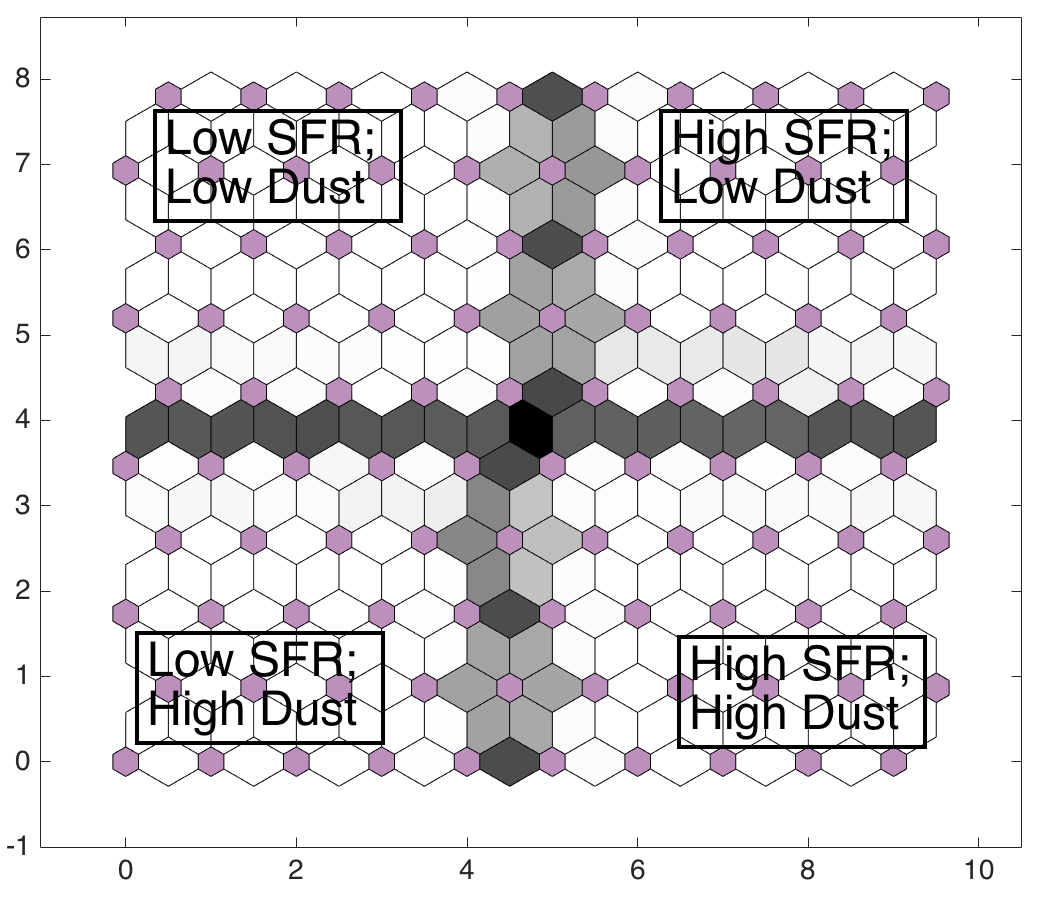
\includegraphics[width=0.5\textwidth]{../images0.01/mock_sample.png}
            \caption{SOM of the mock sample. The axes show the position of the neurons. Hexagonal shapes represent the neurons. The grey-scale colours show the differences between neuron weights, where white is the minimum difference and black is the maximum one.}
            \label{fig: sample}
        \end{figure}
 
To show how self-organizing maps work, we created a mock sample containing only a few regions.
Each sample had two properties: the amount of dust and the star formation rate, where the possible values were
either 0 or 1 for low or high SFR, and 0 or 0.5 for a low or high amount of dust. 
 We generated an SOM from the sample with a size of $10 \times 10$, using the method described in Sec.~\ref{sec: som}.
 Fig. ~\ref{fig: sample} shows the SOM of the mock sample. 
 The axes show the position of the neurons in a $10 \times 10$ network and the hexagonal shapes are the neurons.
 
Using this method, as expected, we are able to divide the mock sample into 4 distinct groups, which their boundaries are shown by grey colours in Fig.~\ref{fig: sample}: regions with high SFR and high dust content, regions with low SFR and high dust content, regions with high SFR and low dust content, and regions with low SFR and dust content. 
The plot in the Fig.~\ref{fig: sample} clearly shows these divisions.
In that plot, the upper part belongs to regions with low dust content, while the lower part belongs to regions with high dust content.
The left part of the plot is where regions with low SFR belong and the right side is for high SFR regions.
Grey to black colours show the border between regions.
This network is considered to be a trained network, and can be used to cluster any new data set with similar entries.

Having two regions with exactly the same values in all their quantities with real data is unprovable. 
If in an input data, there are two entries with similar (but not identical) values in all dimensions, one can find a network that separate these two entries in two groups.  
However, in case of multiple similar entries in data, the number of neurons must be much higher than the number of entries for complete separation.
Therefore, the user learns about similarity/dissimilarity of members of input data based on the ratio of number of entries of input data and number of neurons. 